\documentclass[12pt]{spieman}  % 12pt font required by SPIE;
%\documentclass[a4paper,12pt]{spieman}  % use this instead for A4 paper
\usepackage{amsmath,amsfonts,amssymb}
\usepackage{graphicx}
\usepackage{setspace}
\usepackage{tocloft}

\title{SPIE journal papers: sample manuscript showing style and formatting specifications}

\author[a]{First Author}
\author[a]{Second Author}
\author[b]{Third Author}
\author[a,b,*]{Fourth Author}
\affil[a]{University Name, Faculty Group, Department, Street Address, City, Country, Postal Code}
\affil[b]{Company Name, Street Address, City, Country, Postal Code}

\renewcommand{\cftdotsep}{\cftnodots}
\cftpagenumbersoff{figure}
\cftpagenumbersoff{table} 
\begin{document} 
\maketitle

\begin{abstract}
This document shows the required format and appearance of a manuscript prepared for SPIE journals. It is prepared using LaTeX2e with the class file \texttt{spieman.cls}. Please note that the following journals require the use of structured abstracts in manuscript submissions: \textit{Neurophotonics}, the \textit{Journal of Biomedical Optics}, and the \textit{Journal of Medical Imaging}. Structured abstracts are encouraged for the \textit{Journal of Micro/Nanolithography, MEMS, and MOEMS}. Guidelines are available on the journal website. Whether structured or single-paragraph, the abstract should be a summary of the paper and not an introduction. Because the abstract may be used in abstracting and indexing databases, it should be self-contained (i.e., no numerical references) and substantive in nature, presenting concisely the objectives, methodology used, results obtained, and their significance. A list of up to six keywords should immediately follow. 
\end{abstract}

% Include a list of up to six keywords after the abstract
\keywords{optics, photonics, light, lasers, journal manuscripts, LaTeX template}

% Include email contact information for corresponding author
{\noindent \footnotesize\textbf{*}Fourth author name,  \linkable{myemail@university.edu} }

\begin{spacing}{2}   % use double spacing for rest of manuscript

\section{Introduction}
\label{sect:intro}  % \label{} allows reference to this section
This document shows the format and appearance of a manuscript prepared for submission to SPIE journals. Note that this template is only intended to be used as a guideline for author convenience. It is designed for optimum clarity and ease of reading for editors and reviewers, but the template does not reflect the final page layout of a published journal paper. Accepted papers are professionally typeset in XML according to the layout and design of the journal. 

\subsection{Use of This Document}

This document is prepared using LaTeX2e\cite{Lamport94,Goossens97} with the class file {\ttfamily spieman.cls}.  The LaTeX source file used to create this document is {\ttfamily article.tex}, which contains important formatting information embedded in it. Authors may use it as a template to create their own manuscript. While LaTeX properly handles most formatting issues, the author may occasionally need to intervene to obtain a satisfactorily  formatted manuscript.

\subsection{English}

Authors are strongly encouraged to follow the principles of sound technical writing, as found in Refs.~\citenum{Alred03} and \citenum{Perelman97}, for example. In addition, good English usage is essential. Authors whose native language is not English may wish to collaborate with a colleague whose English skills are more advanced. Alternatively, you may wish to have your manuscript professionally edited prior to submission by Editage, our recommended independent editorial service: \linkable{https://www.editage.com/spie/}. SPIE authors will receive a 15\% discount off their services. A spell checker can be helpful to discover misspelled words, but authors should also proofread their papers carefully prior to submission. Manuscripts that do not meet acceptable English standards or lack clarity may be rejected.

\subsection{Page Setup and Fonts}

All text and figures, including footnotes, must fit inside a text area 6.5 in.\ wide by 9 in.\ high (16.51 by 22.86 cm). Manuscripts must be formatted for US letter paper, on which the margins should be 1 in.\ (2.54 cm) on the top, 1 in.\ on the bottom, and 1 in.\ on the left and right. 

The Times New Roman font is used throughout the manuscript, in the sizes and styles shown in Table~\ref{tab:fonts}. If this font is not available, use a similar serif font. The manuscript should not contain headers or footers. Pages should be numbered.

\begin{table}[ht]
\caption{Fonts sizes and styles.} 
\label{tab:fonts}
\begin{center}       
\begin{tabular}{|l|l|} %% this creates two columns
%% |l|l| to left justify each column entry
%% |c|c| to center each column entry
%% use of \rule[]{}{} below opens up each row
\hline
\rule[-1ex]{0pt}{3.5ex}  Document entity & Brief description  \\
\hline\hline
\rule[-1ex]{0pt}{3.5ex}  Article title & 16 pt., bold, left justified  \\
\hline
\rule[-1ex]{0pt}{3.5ex}  Author names & 12 pt., bold, left justified   \\
\hline
\rule[-1ex]{0pt}{3.5ex}  Author affiliations & 10 pt., left justified   \\
\hline
\rule[-1ex]{0pt}{3.5ex}  Abstract & 10 pt.  \\
\hline
\rule[-1ex]{0pt}{3.5ex}  Keywords & 10 pt.  \\
\hline
\rule[-1ex]{0pt}{3.5ex}  Section heading & 12 pt., bold, left justified  \\
\hline
\rule[-1ex]{0pt}{3.5ex}  Subsection heading & 12 pt., italic, left justified  \\
\hline
\rule[-1ex]{0pt}{3.5ex}  Sub-subsection heading & 11 pt., italic, left justified  \\
\hline
\rule[-1ex]{0pt}{3.5ex}  Normal text & 12 pt. \\
\hline
\rule[-1ex]{0pt}{3.5ex}  Figure and table captions &  10 pt. \\
\hline 
\end{tabular}
\end{center}
\end{table} 

\section{Parts of Manuscript}

This section describes the normal structure of a manuscript and how each part should be handled. The appropriate vertical spacing between various parts of this document is achieved in LaTeX through the proper use of defined constructs, such as \verb|\section{}|. 

\subsection{Title and Author Information}
\label{sect:title}
The article title appears left justified at the top of the first page. The title font is 16 pt., bold. The rules for capitalizing the title are the same as for sentences; only the first word, proper nouns, and acronyms should be capitalized. Do not begin titles with articles (for example, a, an, the) or prepositions (for example, on, by, etc.). The word ``novel'' should not appear in the title, as publication will imply novelty. Avoid the use of acronyms in the title, unless they are widely understood.

The list of authors immediately follows the title, 18 points below. The font is 12 pt., bold and the author names are left justified. The author affiliations and addresses follow the names, in 10-pt., normal font and left justified. For multiple affiliations, each affiliation should appear on a separate line. Superscript letters (a, b, c, etc.) should be used to associate multiple authors with their respective affiliations. The corresponding author should be identified with an asterisk, and that person's email address should be provided below the keywords.

\subsection{Abstract}
The abstract should be a summary of the paper and not an introduction. Because the abstract may be used in abstracting journals, it should be self-contained (i.e., no numerical references) and substantive in nature, presenting concisely the objectives, methodology used, results obtained, and their significance. Please note that the following journals require the use of structured abstracts in manuscript submissions: \textit{Neurophotonics}, the \textit{Journal of Biomedical Optics}, and the \textit{Journal of Medical Imaging}. Structured abstracts are encouraged for the \textit{Journal of Micro/Nanolithography, MEMS, and MOEMS}. Helpful guidelines for structured abstracts are available on the website of the journal.

\subsection{Subject terms/Keywords}
Keywords are required. Please provide 3-6 keywords related to your paper. 

\subsection{Body of Paper}
The body of the paper consists of numbered sections that present the main findings. These sections should be organized to best present the material.

To provide transition elements in your paper, it is important to refer back (or forward) to specific sections. Such references are made by indicating the section number, for example, ``In Sec.\ 2 we showed...'' or ``Section 2.1 contained a description...'' If the word Section, Reference, Equation, or Figure starts a sentence, it is spelled out. When occurring in the middle of a sentence, these words are abbreviated Sec., Ref., Eq., and Fig. 

At the first occurrence of an acronym, spell it out followed by the acronym in parentheses, for example, charge-coupled diode (CCD).

\subsection{Footnotes}
Textual footnotes should be used rarely to present important documentary or explanatory material whose inclusion in the text would be distracting.\footnote{Example of a footnote.} Due to problems with HTML display, use of footnotes should generally be avoided. If absolutely necessary, the footnote mark must come at the end of a sentence. To insert a footnote, use the {\verb|\footnote{}|} command.

\subsection{Appendices}
Brief appendices may be included when necessary, such as derivations of equations, proofs of theorems, and details of algorithms. Equations and figures appearing in appendices should continue sequential numbering from earlier in the paper.

\subsection{Disclosures}
Conflicts of interest should be declared under a separate header. If the authors have no competing interests to declare, then a statement should be included declaring no conflicts of interest. For assistance generating a disclosure statement, see the form available from  the International Committee of Medical Journal Editors website: \linkable{http://www.icmje.org/conflicts-of-interest/} 

\subsection{Code, Data, and Materials Availability}
In support of open scientific exchange, SPIE journals require Data and Code Availability Statements in all accepted papers. This requirement went into effect on 1 May 2023. These statements should describe how to access any data that would be required to replicate or interpret the findings reported in the paper.  

\subsection{Acknowledgments}
Acknowledgments and funding information should be added after the conclusion, and before references. Include grant numbers and the full name of the funding body. The acknowledgments section does not have a section number.

\subsection{References}
The References section lists books, articles, and reports that are cited in the paper. This section does not have a section number. The references are numbered in the order in which they are cited. Examples of the format to be followed are given at the end of this document.

The reference list at the end of this document is created using BibTeX, which looks through the file {\ttfamily report.bib} for the entries cited in the LaTeX source file.  The format of the reference list is determined by the bibliography style file {\ttfamily spiejour.bst}, as specified in the \\ \verb|\bibliographystyle{spiejour}| command.  Alternatively, the references may be directly formatted in the LaTeX source file.

For books\cite{Lamport94,Alred03,Goossens97} the listing includes the list of authors (initials plus last name), book title (in italics), page or chapter numbers, publisher, city, and year of publication.  Journal-article references \cite{Metropolis53,Harris06} include the author list, title of the article (in quotes), journal name (in italics, properly abbreviated), volume number (in bold), inclusive page numbers or citation identifier, and year.  A reference to a proceedings paper or a chapter in an edited book\cite{Gull89a} includes the author list, title of the article (in quotes), conference name (in italics), editors (if appropriate), volume title (in italics), volume number if applicable (in bold), inclusive page numbers, publisher, city, and year.  References to an article in the SPIE Proceedings may include the conference name, as shown in Ref.~\citenum{Hanson93c}.

The references are numbered in the order of their first citation. Citations to the references are made using superscripts, as demonstrated in the preceding paragraph. One may also directly refer to a reference within the text, for example, ``as shown in Ref.~\citenum{Metropolis53} ...''  Two or more references should be separated by a comma with no space between them. Multiple sequential references should be displayed with a dash between the first and last numbers \cite{Alred03,Perelman97,Lamport94,Goossens97,Metropolis53}. 

\subsubsection{Reference linking and DOIs}
A Digital Object Identifier (DOI) is a unique alphanumeric string assigned to a digital object, such as a journal article or a book chapter, that provides a persistent link to its location on the internet. The use of DOIs allows readers to easily access cited articles. Authors should include the DOI at the end of each reference in brackets if a DOI is available. See examples at the end of this manuscript. A free DOI lookup service is available from CrossRef at \\\linkable{http://www.crossref.org/freeTextQuery/}. The inclusion of DOIs will facilitate reference linking and is highly recommended. 

In the present LaTeX template, the author needs to add the DOI reference by including it in a ``note'' in the bibliography file, as shown in the file {\verb+report.bib+}, for example, \\ {\verb+note = "[doi:10.1117/12.154577]"+}. The DOI may be used by the reader to locate that document with the link: {\verb+http://dx.doi.org10.1117/12.154577+}. 

\subsection{Biographies}
A brief professional biography of approximately 75 words may be provided for each author, if available. Biographies should be placed at the end of the paper, after the references. Personal information such as hobbies or birthplace/birthdate should not be included. Author photographs are not published.

\section{Section Formatting}
\label{sect:sections}
In LaTeX, a new section is created with the \verb|\section{}| command, which automatically numbers the sections. Sections will be numbered sequentially, starting with the first section after the abstract, except for the acknowledgments and references. (Note that numbering of section headings is not required, but the numbering must be consistent if used.) All section headings should be left justified.

Main section headings are in 12-pt. bold font, left-justified and in title case, where important words are capitalized.

Paragraphs that immediately follow a section heading are leading paragraphs and should not be indented, according to standard publishing style. The same goes for leading paragraphs of subsections and sub-subsections. Subsequent paragraphs are standard paragraphs, with 0.2-in (5 mm) indentation. There is no additional space between paragraphs. In LaTeX, paragraphs are separated by blank lines in the source file. Indentation of the first line of a paragraph may be avoided by starting it with \verb|\noindent|.

\subsection{Subsection Headings}
All important words in a subsection (level 1) header are capitalized. Subsection numbers consist of the section number, followed by a period, and the subsection number within that section, without a period at the end. The heading is left justified and its font is 12 pt. italic.

\subsubsection{Sub-subsection headings}
The first word of a sub-subsection is capitalized. The rest of the text is not capitalized, except for proper names and acronyms (the latter should only be used if well known). The heading is left justified and its font is 11 pt. italic. 

\section{Figures and Tables}

\subsection{Figures}

Figures are numbered in the order in which they are called out in the text. They should appear in the document in numerical order and as close as possible to their first reference in the text. It may be necessary to move figures or tables around to enhance readability. LaTeX will attempt to place figures at the top or bottom of a page in which they are first referenced.

Figures, along with their captions, should be separated from the main text by  0.2 in.\ or 5 mm and centered. Figure captions are centered below the figure or graph. Figure captions start with the abbreviation ``Fig'' in front of the figure number, followed by a period, and the text in 10-pt. font. See Fig.~\ref{fig:example} for an example.

\begin{figure}
\begin{center}
\begin{tabular}{c}
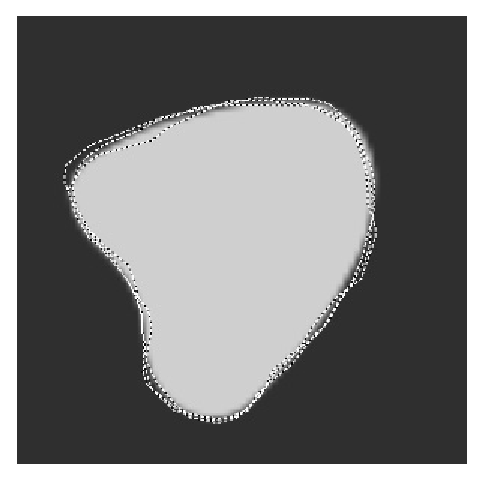
\includegraphics[height=5.5cm]{mcr3b.eps}
\end{tabular}
\end{center}
\caption 
{ \label{fig:example}
Example of a figure caption. } 
\end{figure} 

Authors may wish to create figures consisting of two or more images, in which case, they should be neatly arranged in a rectangular array.  In no case, should the article's text be wrapped around a figure. Figure~\ref{fig:example2} shows two side-by-side images. When a figure contains more than one image, the author must submit them as a single image file. Further details about figure formatting can be found in the author guidelines for each specific SPIE journal: \\
\linkable {https://www.spiedigitallibrary.org/journals/journal-authors}. 

\begin{figure}
\begin{center}
\begin{tabular}{c}

\includegraphics[height=5.5cm]{fig2.eps}  % fig2 includes two images 
\\
(a) \hspace{5.1cm} (b)
\end{tabular}
\end{center}
\caption 
{ \label{fig:example2}
Example of a figure containing multiple images: (a) sun and (b) blob. Figures containing multiple images must be submitted to SPIE as a single image file.} 
\end{figure} 

\subsection{Tables}
Tables are numbered in the order in which they are referenced. They should appear in the document in numerical order and as close as possible to their first reference in the text. It is preferable to have tables appear at the top or bottom of the page, if possible. Table captions are handled identically to those for figures, except that they appear above the table. See Table~\ref{tab:fonts} for an example.

\subsection{Video}
Acceptable file formats, including MOV (.mov), MPEG (.mpg), and MP4 (.mp4), are playable using standard media players, such as VLC or Windows Media Player. The recommended maximum size for each video file is 10-12 MB. Authors may insert a representative still image from the video file in the manuscript as a figure. The caption label will be linked by the publisher to the actual video file. The video may also be mentioned in an existing figure caption. Multimedia files are treated in the same manner as figures and they will be numbered sequentially with normal figures.  The video number, file type, and file size should be included in parentheses at the end of the figure caption. See Figure \ref{vid:satellite} for an example.

\begin{video}
\begin{center}
{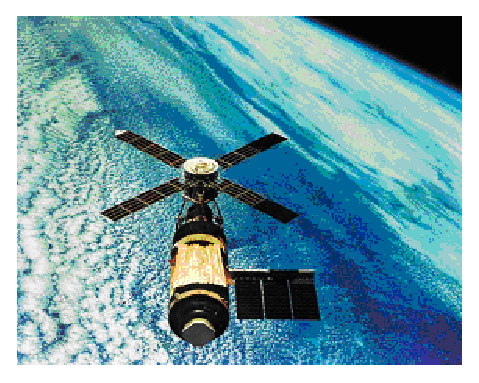
\includegraphics[height=5cm]{satellite.eps}}
\\
\end{center}
\caption{\label{vid:satellite}This satellite is a still image from Video 1 (Video 1, MPEG, 2.5 MB).}
\end{video}

\appendix    % this command starts appendixes

\section{Miscellaneous Formatting Details}
\label{sect:misc}
At times it may be desired, for formatting reasons, to break a line without starting a new paragraph. In a LaTeX source file, a linebreak is created with \verb|\\|.


\subsection{Formatting Equations}
Equations may appear inline with the text, if they are simple, short, and not of major importance; for example, $\beta = b/r$.  Important equations appear on their own line.  Such equations are centered.  For example, ``The expression for the field of view is
\begin{equation}
\label{eq:fov}
2 a = \frac{(b + 1)}{3c} \, ,
\end{equation}
where $a$ is the ...''  Principal equations are numbered, with the equation number placed within parentheses and right justified.  

Equations are considered to be part of a sentence and should be punctuated accordingly. In the above example, a comma appears after the equation because the next line is a subordinate clause. If the equation ends the sentence, a period should follow the equation. The line following an equation should not be indented unless it is meant to start a new paragraph. Indentation after an equation is avoided in LaTeX by not leaving a blank line between the equation and the subsequent text.

References to equations include the equation number in parentheses, for example, ``Equation~(\ref{eq:fov}) shows ...'' or ``Combining Eqs.~(2) and (3), we obtain...'' Note that the word ``Equation'' is spelled out if it begins a sentence, but is abbreviated as ``Eq.'' otherwise. Using a tilde in the LaTeX source file between two characters avoids unwanted line breaks, for example between ``Eq.'' and the following equation number..

\subsection{Formatting Theorems}

To include theorems in a formal way, the theorem identification should appear in a 10-point, bold font, left justified, and followed by a period.  The text of the theorem continues on the same line in normal, 10-pt. font, achieved in LaTeX using \verb|\footnotesize|.  For example, 

\vspace{2ex}\noindent{\footnotesize\textbf{Theorem 1.} For any unbiased estimator...}

% \disclosures 
\subsection*{Disclosures}
Conflicts of interest should be declared under a "Disclosures" header. If the authors have no relevant financial interests in the manuscript and no other potential conflicts of interest to disclose, a statement to this effect should also be included in the manuscript.


\subsection* {Code, Data, and Materials Availability} 
In support of open scientific exchange, SPIE journals require Code, Data, and Materials Availability Statements in all accepted papers. This requirement went into effect on 1 May 2023. These statements should describe how to access any data that would be required to replicate or interpret the findings reported in the paper. Authors are encouraged to make the data and code related to the manuscript publicly available whenever possible, and utilize repositories that are well-known to the field (FigShare, Github, CodeOcean, etc.). If the data or code cannot be made publicly available, the authors should state the reason and explain how it can be obtained. Likewise, if data sharing is not applicable, the statement must say so. Example statements may be found in the Author Guidelines for the journal.


\subsection* {Acknowledgments}
This unnumbered section is used to identify those who have aided the authors in understanding or accomplishing the work presented and to acknowledge sources of funding. 


%%%%% References %%%%%

\bibliography{report}   % bibliography data in report.bib
\bibliographystyle{spiejour}   % makes bibtex use spiejour.bst

%%%%% Biographies of authors %%%%%

\vspace{2ex}\noindent\textbf{First Author} is an assistant professor at the University of Optical Engineering. He received his BS and MS degrees in physics from the University of Optics in 1985 and 1987, respectively, and his PhD degree in optics from the Institute of Technology in 1991.  He is the author of more than 50 journal papers and has written three book chapters. His current research interests include optical interconnects, holography, and optoelectronic systems. He is a member of SPIE.

\vspace{1ex}
\noindent Biographies and photographs of the other authors are not available.

\listoffigures
\listoftables

\end{spacing}
\end{document}